\documentclass[../manuscript.tex]{subfiles}

\section{Введение}
\subsection{Представление химических веществ}
Проблема представления химических молекул в виде, пригодном для анализа и обработки на компьютере, является острой. В современной хемоинформатике используется множество различных представлений химических молекул таких как: номенклатурное представление, линейные нотации, различные матричные представления. Так как каждый из форматов имеет свои сильные и слабые стороны, не существует единого стандарта хранения химических соединений. Более того, для различных задач используются различные форматы. В данной главе будут рассмотрены основные представления химических веществ и форматы их хранения.


\subsubsection{Линейная нотация}
Наиболее популярными среди линейных нотаций молекул являются следующие: Wiswesser (WLN), ROSDAL, SMILES и Sybyl (SLN) \cite{Gasteiger2003}. Большинство из вышеперечисленных нотаций в настоящее время используются редко, поэтому имеет смысл подробно остановиться только на нотации SMILES. 

\begin{itemize}
    \item SMILES (Simplified Molecular Input Line Entry System)
        \newline
        Данная нотация получила широкое распространение и применяется повсеместно для хранения химических молекул. SMILES основана на шести простых правилах представления молекул:
        \begin{itemize}
            \item Атомы представлены своими химическими символами
            \item Атомы водорода автоматически заполняют свободные валентности и опускаются
            \item Соседние атомы расположены подряд
            \item Двойная и тройная связи представляются символами "$=$" и $"\#"$ соответственно
            \item Боковые цепи молекулы заключаются в скобки
            \item Атомы циклов, находящиеся на концах разорванной при построении линейной нотации молекулы, обозначаются одним и тем же номером
        \end{itemize}
\end{itemize}
\par Данный вариант представления химических структур имеет ряд достоинств: наиболее простое линейное представление, возможность быстрого обмена данными, поддержка структуры Маркуша, стереохимии и некоторых других опций. Однако существует несколько серьезных недостатков данного формата: неоднозначность декодирования, а также некоторые проблемы с представлением ароматических соединений.

\par В настоящее время существует множество разновидностей форматов SMILES. Наиболее интересным для текущей задачи является формат USMILES (Unique SMILES), позволяющий однозначно восстанавливать химическую структуру молекул после конвертации из формата USMILES. 


\subsubsection{Молекулярный граф}
Часто молекулы представляются в виде молекулярных графов. Под термином молекулярный граф мы понимаем следующее: молекулярный граф — связный неориентированный граф, находящийся во взаимно-однозначном соответствии со структурной формулой химического соединения таким образом, что вершинам графа соответствуют атомы молекулы, а рёбрам графа — химические связи между этими атомами. Как правило в органической химии при представлении молекул опускаются атомы водородов, а также символы атомов углеродов.

\par В компьютере молекулярные графы часто представляются в виде матриц. На \hyperref[pic1.sec3.1.2]{рисунке ниже} показано, как молекулярный граф представляется в виде матрицы. Каждому атому присваивается уникальный номер. Если два атома, например атом 1 и атом 5 \hyperref[pic1.sec3.1.2]{на рисунке}, связаны, то в матрице в полях [1,5] и [5,1] будет стоять единица, в противном случае, если атомы не связаны, стоит ноль.
\begin{figure}[H]
\label{pic1.sec3.1.2}
    \centering
    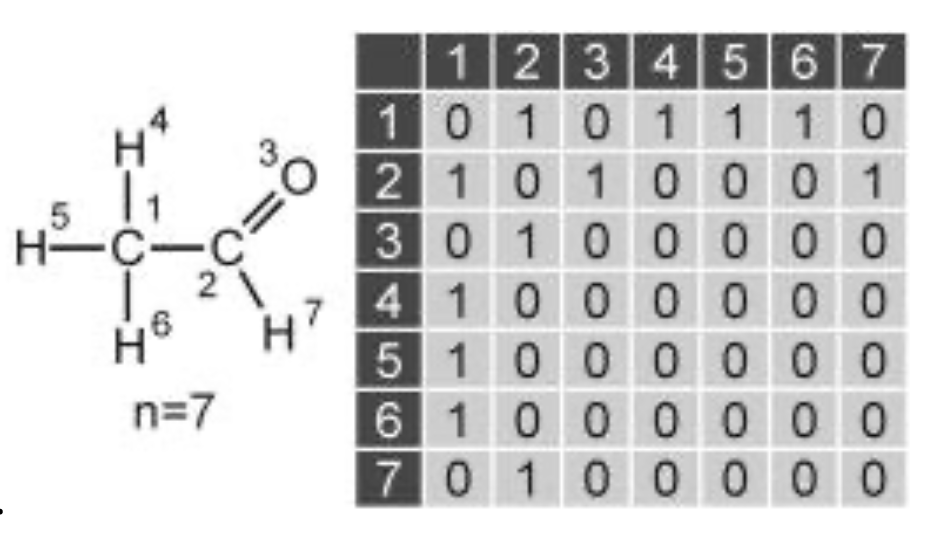
\includegraphics[scale=0.6]{pic_1_sec_3.1.2.png}
    \caption{Представление молекулярного графа в виде матрицы}
\end{figure}

\subsubsection{Матричное представление молекул}
В настоящее время широко используется матричное представление молекул. Существует множество различных матриц, таких как: матрицы смежности, матрицы расстояний, матрицы связей и т.д. Несмотря на разнообразие матриц, существует два основных принципа матричного представления молекул: каждая молекула представлена в виде матрицы $ n \times n $, где n - число атомов молекулы; каждый атом описывается дважды - в столбце и в строке матрицы.

\begin{itemize}
    \item Матрица смежности
    \newline
    Матрица смежности молекулы - квадратная матрица размера $ n \times n $, показывающая все связи между атомами. Единица, стоящая на пересечении строки i и столбца j означает, что атомы с номерами i и j соединены. В противном случае на пересечении строк стоит 0. На диагонали матрицы всегда стоят нули.
   \newline
   Данная матрица может рассматриваться как обобщение матрицы связей. Содержит дополнительную информацию о числе свободных валентных электронов на конкретном атоме диагональных элементов.
\end{itemize}


\par В целом матричное представление молекул обладает рядом плюсов и минусов. Из достоинств можно отметить, что молекулярный граф полностью кодирует молекулу, а также позволяет применять матричную алгебру. Существенным недостатком является тот факт, что число значений возрастает пропорционально $n^2$, а также не учитывается стереохимия молекул.


\subsubsection{Таблица связей}
Для решения проблемы матричного представления и квадратичного возрастания значений при увеличении числа атомов в молекуле был предложен метод представления молекул, под названием таблица связей. Данная структура представляет собой два списка один из которых: список всех атомов молекулы и таблица из трех столбцов. Первые два столбца таблицы показывают какие атомы связаны между собой, а третий столбец - порядок связи (одинарная = 1, двойная = 2 и т.д.). Как и в большинстве других представлений молекул, атомы водорода в большинстве случаев опускаются и при визуализации молекул восстанавливаются по стандартной валентности атомов. Структура таблицы связей может быть дополнена различными списками, такими как списки свободных электронов или список зарядов атомов молекул. 


\par Такой формат представления молекул имеет ряд существенных преимуществ над описанными выше, такие как: число значений растет  линейно с увеличением числа атомов в молекулах, возможно добавление дополнительной информации о молекуле, помимо атомов и связей. Более того, данное представление широко используется в множестве различных пакетов для работы с химическими данными. 

\subsubsection{Форматы файлов для хранения химических данных}
\par В настоящее время существует большое число форматов файлов для хранения разнообразных химических данный. В данной главе будут освещены основные форматы:
\begin{itemize}
    \item Molfile
    \newline
    Формат данных Molfille является одним из наиболее используемых форматов для хранения структуры химических молекул. Данный формат хранит молекулы в виде таблицы связей. Основным недостатком этого формата является отсутствие единого формата таблиц связей. Расширение данного файла: *.mol
    \item SMILES
    \newline
    Также широко распространенный формат файла. Данный формат хранит линейную нотацию молекул. Расширение файлов: *.smi
    \item PDB file
    \newline
    Данный формат файла используется для хранения 3D структур биологических макромолекул. Расширение фойлов: *.pdb
    \newline
    \item CIF
    \newline
    Данный формат используется для хранения 3D структур молекул, полученных методом кристаллографии. Расширение файлов: *.cif
    \item JCAMP
    \newline
    Данный формат используется для хранения информации о молекуле, полученной методом спектрометрии. Существует две модификации данного формата: первая, JCAMP-CS, содержит структурную информацию о молекулах и является аналогом Molfile; вторая, JCAMP-DX, непосредственно содержит спектроскопические данные о молекуле. Расширения фалов: *.jdx, *.dx, *.cs
    \item CML
    \newline
    Данный формат файла является неким обобщением всех вышеперечисленных. В данном формате собрана вся химическая информация о молекуле, доступная на текущий момент. Расширение файлов: *.cml
\end{itemize}
\subsubsection{Однозначное и единственное представление молекул}
Все вышеперечисленные представления молекул обладают одной существенной проблемой, которая на практике затрудняет применение этих представлений: неоднозначность обратного преобразования молекулы в структурную формулу и множественность представления структурной формулы в виде, например, таблицы связей. Более того, для каждой молекулы, состоящей из n атомов, имеется $ n! $ различных ее представлений в виде таблицы связей.

\par Для решения этой проблемы в большинстве случае применяют алгоритм Моргана. Этот алгоритм позволяет однозначно кодировать и декодировать химические вещества, а также учитывать их стереохимию. 
\par Алгоритм Моргана состоит из двух основных частей: процесса релаксации, который классифицирует атомы в зависимости от их соседей, и присваивания уникальных и инвариантных номеров атомам. Далее более подробно будут описаны эти процессы.

\begin{itemize}
    \item \textit{Классификация атомов по их соседям (процесс релаксации)}
    \newline
    На данном этапе происходит подсчет extended connectivity (EC), на основе которых атомам присваиваются уникальные номера.
    \item \textit{Присваивание каждому атому уникального инвариантного номера}\newline
    На этом этапе атомам присваиваются уникальные номера. Атому с наибольшим EC, полученным на последней итерации предыдущего этапа, присваивается номер 1. Номер 2 получает атом, связанный с атомом 1, с наибольшим значением EC. Дальнейшая нумерации строится аналогично. После нумерации всех атомов, связанных с первым, нумерация продолжается с еще не пронумерованных соседей атома 2 и так далее. Если при нумерации встречаются атомы с одинаковыми значениями EC, то дальнейшая нумерация подчиняется строгим правилам, которые учитывают тип атом, его связи, заряд и так далее.
\end{itemize}
\subsubsection{Фрагментное кодирование молекул}
\par Ещё одним распространенным способом представления молекул является фрагментное кодирование, а именно фингерпринты. Для этого молекула разбивается на отдельные функциональные группы, кольца и так далее. Структурные фингерпринты представляют собой бинарные последовательности нулей и единиц, которые показывают наличие (1) или отсутствие (0) какой-либо подструктуры в описываемой молекуле. Стандартный размер структурного фингерпринта - 150-2500 бит. Такое простое представление молекулы в виде строки позволяет легко находить сходства между молекулами и осуществлять поиск близких по структуре молекул.

\par Кроме того, структурные фингерпринты могут подвергаться хэшированию - преобразованию по специальному алгоритму в строку строго определенной длины. С хэшированными фингерпринтами удобнее работать, их быстрее сравнивать и быстрее производить поиск, так как их длина строго фиксирована. Более того, так как при появлении в молекуле каждый отдельный фрагмент активирует не одну позицию в фингерпринте, а сразу несколько, то вероятность "коллизии" достаточна низкая, чтобы по такого рода фингерпринтам однозначно восстанавливать структурную формулу молекулы. На \hyperref[pic1.sec3.1.7]{рисунке ниже} приведен наглядный пример того, что было описано выше.
\begin{figure}[H]
\label{pic1.sec3.1.7}
    \centering
    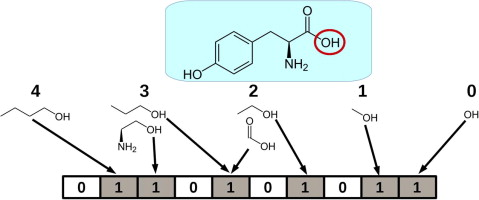
\includegraphics[scale=0.6]{pic_1_sec_3.1.7.jpg}
    \caption{Пример построения хэшированного фингерпринта}
\end{figure}
%\par Помимо структурных фингерпринтов существуют еще и так называемые "хэшированные фингерпринты". Данный вид фингерпринтов отличается от структурных тем, что молекула разбивается на куски определенной длины, а не на отдельные структурные элементы, и хранится в виде последовательности нулей и единиц в зависимости от наличия или отсутствия определенного куска. 
%\newline
\par Подводя итог данной части, хотелось бы отметить, что существует множество разнообразных представлений молекул, каждое из которых подходит под строго определенные цели и задачи. В этой работе будут использованы такой формат файлов, как SMILES, а также фингерпринты Моргана для поиска сходства молекул.

\subsection{Топология биологических сетей}
В настоящее время различные биологические сети получили широкое распространение. Существует несколько основных видов биологических сетей:
\begin{itemize}
    \item сети белок-белковых взаимодействий
    \item генные сети
    \item сети метаболических путей
\end{itemize}
\par В данном разделе будут подробно рассмотрены все виды сетей, а также освещены основные метрики, используемые при работе с биологическими сетями.
\subsubsection{Сети белок-белковых взаимодействий}

Данный вид сетей представляет собой ненаправленный граф, вершинами которого являются белки. Две вершины соединены ребром, если два соответствующих белка взаимодействуют между собой в биологической системе.
Сети такого рода являются по своему строению безмасштабными сетями, то есть степени вершин таких сетей распределены по степенному закону, то есть доля вершин со степенью $k$ примерно или асимптотически пропорциональна $k^{-\gamma }$.

\par Для работы с такими сетями было предложено множество различных метрик центральности, таких как: 
\begin{itemize}
    \item степень вершины (degree) - число ребер графа, которым принадлежит эта вершина $$ d_i = \sum\limits_j u_j ,$$ где $u_j$ - ребро графа, принадлежащее данной вершине.
    
    \item кратчайшее расстояние между вершинами (shortest distance) - минимальное число ребер невзвешанного графа, которое нужно пройти, чтобы попасть из одной вершины в другую.
    
    \item степень посредничества (betweenness) - это мера центральности в графе, основанная на кратчайших путях. Для любой пары вершин в связном графе существует по меньшей мере один (кратчайший) путь между вершинами, для которого минимально либо число рёбер, по которым путь проходит, (для невзвешенных графов), либо сумма весов этих рёбер (для взвешенных графов). Степень посредничества для каждой вершины равна числу этих кратчайших путей через вершину, нормированных на общее число кратчайших путей в графе. $$ g(v) = \sum\limits_{s \neq v \neq t} \frac{\sigma_{st}(v)}{\sigma_{st}} ,$$ где  $\sigma _{st}$ равно общему числу кратчайших путей из узла s в узел t, а $\sigma _{st}(v)$ равно числу этих путей, проходящих через v.
    
    \item связанность (connectivity) - минимальное число элементов графа (вершин и ребер), которое необходимо удалить, чтобы разделить оставшиеся вершины на изолированные подграфы.
    
    \item cтепень близости узла (к другим узлам) (closeness) — это мера центральности в сети, вычисляемая как обратная величина суммы длин кратчайших путей между узлом и всеми другими узлами графа. Таким образом, чем более централен узел, тем ближе он ко всем другим узлам. $$C(x)={\frac  {1}{\sum _{y}d(y,x)}} ,$$ где $d(x,y)$ - расстояние между вершинами x и y.
    
    \item степень влиятельности (eigenvector centrality) - метрика центральности графа, вычисляемая как собственные вектора матрицы смежности.
    Решается уравнение на поиск собственных векторов матрицы: $$\textbf{Ax} = \lambda \textbf{x} ,$$
    где \textbf{A} - матрица смежности, \textbf{x} - собственный вектор, а $\lambda$ - собственное значение матрицы смежности, соответствующее данному собственному вектору. Также это векторное уравнение можно переписать в виде суммирования по всем вершинам: $$x_{v}={\frac {1}{\lambda }}\sum _{t\in M(v)}x_{t}={\frac {1}{\lambda }}\sum _{t\in G}a_{v,t}x_{t},$$
    где $M(v)$ представляет собой множество соседей вершины v, а $ \lambda$  является константой. 
    \item центральность графа Харари (Harary graph centrality) для вершины (v) определяется формулой: $$C(v) = {1 \over {max_u d(v, u)}},$$ где $d(v, u)$ - кратчайшее расстояние между вершинами v и u.
    
    \item информационная центральность (information centrality) - средняя гармоническая длина путей, заканчивающихся в вершине s. Чем больше у вершины s коротких путей, соединяющих ее с другими вершинами, тем меньше данная метрика.
    Сначала определим понятие Матрица Кирхгофа: $$\textbf{L} = \textbf{D} - \textbf{A},$$
    где \textbf{A} - взвешанная матрица смежности графа, \textbf{D} - диагональная матрица такая, что $${ d_{i,j}:={\begin{cases}\deg(v_{i})&{\text{при}}\ i=j,\\0&{\text{в противном случае}}.\end{cases}}}$$
    Тогда $${l_{i,j}:={\begin{cases}\deg(v_{i})&{\text{при}}\ i=j,\\-1&{\text{при}}\ (v_{i},v_{j})\in E(G),\\0&{\text{в противном случае}}.\end{cases}}}$$
    Определим матрицу \textbf{J} как матрицу всех вхождений, которые равны единице. Определим матрицу \textbf{B} как $\textbf{B} = \textbf{L} + \textbf{J}$. Тогда определим информацию, проходящую между вершинами $u$ и $v$ как $$ I_{uv} = \frac{1}{\textbf{B}^{-1}(u,u) + \textbf{B}^{-1}(v,v) - 2\textbf{B}^{-1}(u,v)}$$
    Тогда информационной центральностью называется гармоническое среднее $I_{uv}$ по всем вершинам $u$: $$I_v = \frac{n}{\sum\limits_{u \in V} \frac{1}{I_{uv}}}.$$
    
    \item stress центральность (stress centrality) - простая сумма числа всех кратчайших путей, проходящих через вершины. $$ C_s(v) = \sum\limits_{s \neq t \neq v \in V} \rho_{st}(v) , $$ где $\rho_{st}(v)$ - число кратчайших путей, проходящих через вершину $v$.
    
    \item центральность близости вершин при случайном блуждании  (random walk closeness) - это мера центральности сети, которая описывает среднюю скорость, с которой случайно идущие процессы достигают узла из других узлов сети.

    Рассмотрим взвешенный граф (направленный или ненаправленный) с $n$ вершинами, обозначенными $j = 1,…, n;$ и процесс случайного блуждания по этому графу с матрицей перехода M. Элемент $m _ {{jk}}$ в M описывает вероятность случайного блуждания из вершины i перейти непосредственно в вершину j . Эти вероятности определяются следующим образом. $$ M (i, j) = { \frac{a_ {ij}}{\sum_{j = 1}^{n} a_{ij}}},$$
    где $a_{{ij}}$ - это (i, j)-й элемент матрицы весов графа A. Когда между двумя вершинами графа нет ребра, то соответствующий элемент матрицы A равен нулю.
    
    Центральность близости случайного блуждания вершины i является обратной величиной среднего времени первого перехода к этому узлу: $$ C_{i}^{RWC} = {\frac{n}{\sum_{j = 1}^{n} H(j, i)}}$$
    Среднее время первого прохождения от вершины i к вершине j - это ожидаемое количество шагов, которое потребуется процессу, чтобы впервые достичь узла j из узла i: $$ H (i, j) = \sum_{r = 1}^{\infty} rP(i, j, r),$$
    где $P(i, j, r)$ - вероятность того, что требуется ровно r шагов, чтобы достичь j из i в первый раз. Чтобы вычислить эти вероятности достижения вершины в первый раз за r шагов, полезно ввести преобразование M путем удаления его j-ой строки и столбца; обозначим его как $M_{- j}$. Поскольку вероятность того, что процесс начнется с i и окажется в k после r-1 шагов, просто является (i, k)-м элементом ${M_{-j}^{r-1}}$, $P(i, j, r)$ можно выразить как $$P( i, j, r) = \sum_{k \neq j} ((M_{- j}^{r-1}))_{ik} m_{kj}$$
    Подставляя это в выражение для среднего времени первого прохождения, получаем $$H (i, j) = \sum_{r = 1}^{\infty} r \sum_{k \neq j} ((M_{- j}^{r -1}))_{ik} m_{kj}$$
    Используя формулу суммирования геометрических рядов для матриц, получаем $$H (i , j) = \sum_{k \neq j} ((I-M_{- j})^{- 2})_{ik} m_{kj}$$
    где I - это n-1-мерная единичная матрица.
    
    \item центральность посредничества вершин при случайном блуждании (random walk betweenness) - по существу тоже самое, что и посредничество, однако вместо кратчайших путей используются случайные блуждания из одной вершину в другу. $$C_{i}^{RWB}=\sum _{j\neq i\neq k}r_{jk},$$ где элемент $r_{jk}$ матрицы R, который содержит вероятность случайного блуждания, начинающегося в узле j с поглощающим узлом k, проходящего через узел i.
    
    \item коэффициент кластеризации (clustering coefficient) - это мера того, в какой степени узлы в графе склонны группироваться вместе. Существуют две версии этой меры: глобальная и локальная. Глобальная версия была разработана для того, чтобы дать общее представление о кластеризации в сети, тогда как локальная показывает вовлечённость отдельных узлов.
    
    Предположим, что граф полностью описывается матрицей смежности A. Тогда локальный коэффициент кластеризации i-ой вершины графа можно рассчитать следующим образом:
    $$C_{i}={\frac {1}{k_{i}(k_{i}-1)}}\sum _{j,k}A_{ij}A_{jk}A_{ki}, $$ где $k_{i}=\sum _{j}A_{ij}$.
    Глобальный коэффициент кластеризации всего графа может быть рассчитан по следующей формуле: $$C={\frac {\sum _{i,j,k}A_{ij}A_{jk}A_{ki}}{\sum _{i}k_{i}(k_{i}-1)}},$$ где $k_{i}=\sum _{j}A_{ij}$.
    
    \item центральность подграфа (subgraph centrality) вершины показывает количество подграфов, в которых содержится данная вершина, нормализуя метрику на размеры подграфов.
    Определим локальный спектральный момент матрицы смежности $\textbf{A}$ как i-ый диагональный элемент k-ой степени матрицы смежности:$$\mu_k(i) = (\textbf{A}^k)_{ii}$$ Тогда центральность подграфа будем называть следующее выражение: $$SC(v) = \sum\limits_{k = 0}^{\infty} \frac{\mu_k(v)}{k!}$$
    
    \item центральность близости Фримена (Freeman closeness) - полное геодезическое расстояние от данной вершины до всех других . Данная метрика определяется следующей формулой: $$C(v) = \frac{1}{\sum_{i\neq v}d(v,i)},$$ где $d(v, i)$ - кратчайшее расстояние между вершинами v и i.
    
\end{itemize}

\newpage
\par Также довольно часто используются метрики консервативности белков, как мера их важности:
\begin{itemize}
     
     \item эволюционное расстояние D определяется формулой \newline 
     $$ q = \ln{\frac{1 + 2D}{2D}},$$ где q - отношение числа консервативных сайтов в последовательности выравниваний пар белков
    \item ESC (excess sequence conservation) - средняя избыточная последовательность является мерой эволюционной консервативности белка. Определяется следующим соотношением:$$\left\langle ESC_k \right\rangle = {1 \over N_k} \sum\limits_i ^{N_k} \frac{\left\langle D \right\rangle - D_i}{\left\langle D \right\rangle},$$ где $N_k$ - количество белков в соответствующей группе k, а $ \left\langle D \right\rangle = {1 \over N}\sum\limits_i ^{N} D_i$ - среднее эволюционное расстояние всех N белков
    \item ER (excess retension): 
    В соответствии со степенью вершины k в базовой сети взаимодействия белков все белки группируются в ячейки по логарифмически увеличивающейся связности k. В каждой ячейке отношение $e^A_k = {n^A_k \over N_k}$ представляет собой определенную характеристику A, где $n^A_k$ - это количество белков, которые имеют характеристику A (например, являются незаменимыми или ортологичными в эталонном организме), а 
    $N_k$- общее количество белков. В отсутствии корреляции между A и его положением в сети, $e^A_k$ имеет общее значение, не зависящее от k, $e = {n \over N}$, где $n = \sum_k n^A_k$ - общее количество белков организма, имеющих признак A, а $N = \sum_k N_k$ - общее количество белков в основной сети. Таким образом, для каждой группы k мы определяем эволюционное избыточное удержание признака A как $ER^A_k = {e^A_k \over e}$, которое должно иметь независимое от k значение $ER_k = 1$ при случайном присвоении A.
\end{itemize}

\par Вопрос выбора метрики для определения важности белков до сих пор остается нерешенным, поэтому актуальной является задача подбора оптимальных метрик для решения конкретных задач на конкретных данных. В литературе существует множество статей, которые описывают процесс подбора метрик для конкретного исследования, что подтверждает описанную выше проблему выбора метрики.

\par  Jeong et al. \cite{jeong2001} описали идею использования такой топологической метрики, как степень вершины графа белок-белковых взаимодействий для определения летальность мутации того или иного белка сети в дрожжах Saccharomyces cerevisiae. Мутации моделировались путем исключения случайной вершины из графа взаимодействий. Полученные результаты валидировались на списке известных летальных мутаций для дрожжей. Было показано, что белки с высокой степенью вершины в 3 раза вероятнее окажутся важными для выживаемости организма, нежели белки с низкой степенью вершины. Однако, существует противоположная точка зрения, опровергающая связь топологических метрик центральности и важности белков. Утверждается, что для важных белков накоплено больше данных, чем для редких белков, поэтому связь топологических метрик с важностью белка ставится под сомнение.

\par Hahn et al. \cite{hahn2005} подробно описали использование трех метрик центральности, таких как связанность, степень посредничества и степень близости узла, для определения важности белков, а также их эволюционной консервативности в трех эукариотических организмах: Saccharomyces cerevisiae, Caenorhabditis elegans и Drosophila melanogaster. В датасет для построения сетей белок-белковых взаимодействий вошли только те белки, которые имеют ортологов во всех трех организмах. Полученные результаты валидировались на результатах более ранних исследований, в которых была выявлена летальность того или иного белка. Было показано, что белки с высокой степенью вершины в 3 раза вероятнее окажутся важными для выживаемости организма, нежели белки с низкой степенью вершины. Было показано, что положение белка в сети белок-белковых взаимодействий влияет как на скорость его эволюционных изменений, так и на вероятность оказаться важным для выживаемости. Также стоит отметить, что для необходимых генов все три метрики были выше, чем для остальных, что подтверждает наличие корреляции между центральностью белков в сети взаимодействий и их важностью для выживания организма.

\par Pržulj et al. \cite{prvzulj2004} исследовали такие метрики, как связанность, длина кратчайшего пути и количество точек сочленения. Был проведен систематический анализ, основанный на теории графов сети белок-белковых взаимодействий для построения вычислительных моделей для описания и прогнозирования свойств летальных мутаций и белков, участвующие в генетических взаимодействиях, функциональных групп, белковых комплексов и сигнальных путей.
Анализ показал, что летальные мутации не только
сильно связаны в сети, но и обладают дополнительным свойством: их удаление вызывает нарушение целостности сети. Также были предоставлены доказательства существования альтернативных путей обхода жизнеспособных белков сети, в то время как подобных путей для летальных мутаций не существует.
Кроме того, было установлено, что разные функциональные классы белков обладают разными характеристиками сети. Во время валидации была оценена весомость прогнозов путем их сравнения со случайной моделью, и оценена точность прогнозов за счет анализа их перекрытия с базой данных \href{http://mips.helmholtz-muenchen.de/proj/ppi/}{MIPS}.
\par Joy et al. \cite{joy2005} исследовали такие метрики центральности графа, как степень посредничества и связанность для исследования структуры сетей белок-белковых взаимодействий. В проделанной работе была уточнено строение белковый сетей, а именно был найден такой вид вершин, как HBLC (high betweenness and low connectivity), то есть вершины с высоким значением степени посредничества и низким значением связанности. Однако ранее считалось, что существуют лишь два типа вершин графов белок-белковых взаимодействий: вершины с низкой степенью посредничества и низкой связанностью и наоборот - вершины с высокими значениями обеих метрик.

\par Прежде чем описывать дальнейшие результаты, стоит описать вычислительные модели эволюции биологических сетей, использовавшиеся для валидации полученных данных.
\begin{itemize}
    \item Модель Барабаши — Альберт (BA модель)
    \newline
     Алгоритм генерации случайных безмасштабных сетей с использованием принципа предпочтительного присоединения. Сеть начинается с начальной сетки с $ m_{0}$ узлами. $m_{0}>=2$ и степень каждого узла в начальной сети должна быть не меньше 1, иначе она всегда будет отделена от остальной части сети.
    В каждый момент времени в сеть добавляется новый узел. Каждый новый узел соединяется с существующими узлами с вероятностью, пропорциональной числу связей этих узлов. Формально, вероятность $p_{i}$ того, что новый узел соединится с узлом i, равна:$$p_{i}={k_{i} \over \sum _{j}k_{j}},$$
    где $k_i$ — степень i-го узла, а в знаменателе суммируются степени всех существующих узлов. Наиболее связанные узлы («хабы»), как правило, накапливают ещё больше связей, тогда как узлы с небольшим числом связей вряд ли будут выбраны для присоединения новых узлов. Новые узлы имеют «предпочтение» соединяться с наиболее связанными узлами. Такой принцип связывания узлов называется принципом предпочтительного соединения.
    
    \item Обобщенная модель Барабаши - Альберт (EBA модель)
    \newline
    По сути явлияется обобщением модели BA, где добавление соединений и их изменение происходит вместе с добавлением узлов с преимущественным присоединением.
    
    \item Модель Sole - Vazquez (SV модель)
    \newline
    Биологически ориентированная модель построения безмасштабных сетей. 
    В этой модели существующие узлы (белки) копируются со всеми их существующими связями, за чем следует дивергенция дублированных узлов, вводимая путем изменения связей и/или добавления связей, имитируя мутации дублированных генов.
    
    \item Модель дупликация-мутация (DM модель)
    \newline
    Биологически ориентированная модель построения безмасштабных сетей, учитывающая дупликации и мутации генов. Точечные мутации, которые влияют на способность белка участвовать в молекулярных взаимодействиях, моделируются как присоединение или отсоединение связей, в то время как количество узлов фиксировано («динамика связей»). Поскольку дублирование узлов в эволюционных временных масштабах происходит медленно, по сравнению с временной шкалой динамики связей, дублирование генов моделируется как добавление узлов без каких-либо связей, в то время как динамика связей происходит на каждом временном шаге. Это было оправдано наблюдением, что в дублированных генах полная диверсификация происходит почти сразу после дупликации. Обычно это расхождение является необъективным, так как один из белков сохраняет большую часть взаимодействий, в то время как другой сохраняет несколько или ни одного. Таким образом, для динамики связи в нашем моделировании новое присоединение устанавливается следующим образом: выбирается случайный узел и присоединяется к другому узлу с предпочтительным присоединением, то есть со скоростью, пропорциональной его связанности k, как в модели BA. Напротив, для отсоединения связь между двумя узлами выбирается со скоростью отсоединения, пропорциональной сумме инверсий их связностей. Это мотивировано наблюдением более высокой частоты мутаций для менее связанных белков. 
\end{itemize}

\par При анализе четырех существующих вычислительных моделей эволюции биологических сетей (BA модель, EBA модель, SV модель и DM(duplication-mutation) модель) было установлено, что только модель DM способна воспроизводить сети, содержащие HBLC белки. Сравнивая модели роста сети, было обнаружено, что мутации (изменения в сетевых связях из-за их добавления и удаления) играют центральную роль в механизме создания сети, вследствие чего появляются HBLC белки. Таким образом, предложенный алгоритм объясняет эту отличительную черту топологии сети без необходимости учета функциональной адаптации. В этом исследовании показано, что существование белков HBLC является неизбежным следствием определенных молекулярных механизмов роста сети, которые включают в себя случайные изменения схемы связи из-за мутаций. Это, вместе с открытием того, что узлы HBLC, по-видимому, не являются эволюционно более старыми белками, поддерживает идею о том, что присутствие белков HBLC обусловлено внутренними, структурными и механистическими ограничениями роста сети.

\par Park et al.\cite{park2009} рассмотрели 40 различных метрик центральности, относящихся как к глобальным или локальным, так и метрики, ранее не рассматривавшиеся для оценки центральности в графах белок-белковых взаимодействий. Были рассмотрены две сети взаимодействий для белков дрожжей, полученных из разных баз данных. Результаты показали, что измерения центральности информации на основе маршрута и локализованной информации предсказывают важность белков в обеих сетях. И наоборот, предполагается, что меры глобальной центральности и меры, связанные с хабами (наиболее центральными белками сети), могут не подходить для выявления значимости белков. Кроме того, меры центральности локальной информации, охватывающие различные диапазоны, предоставляют релевантную информацию о важных узлах. Меры локализованной центральности, которые предполагают идеальные пути или случайные блуждания, показывают более слабую корреляцию со значимостью белков, чем меры информационной центральности. То есть те меры центральности, которые представляют сложность окружающей среды и учитывают локальную подсеть вокруг конкретного узла, являются лучшими мерами для прогнозирования важных узлов в сети белок-белковых взаимодействий. Основываясь на выводе о том, что меры центральности локализованной информации содержат наиболее важную информацию для прогнозирования существенности, был сделан вывод, что локальные плотные кластеры содержат важные узлы, поскольку влияние возмущения на кластеры может быть значительным на основаниях предположения, что сигнал проходит через несколько путей, использующих окружающую вершину среду, а не только кратчайший путь. Кроме того, результаты анализа кластеризации показывали, что определенные биологические процессы ассоциируются с определенными сетевыми кластерами, предполагая тесную взаимосвязь между конкретной топологией сети и биологической функцией. В заключение, было продемонстрировано, что клеточные функции, включая важность белков, тесно связаны с топологией сети.
 
\par Помимо топологических метрик центральности сетей белок-белковых взаимодействий Wuchty et al.\cite{wuchty2004} рассмотрели так называемые эволюционные метрики консервативности белков. В работе была предложена новая эволюционная метрика ER(evolutionary retention), которая позволяет выявить устойчивую и сильную корреляцию между консервативностью, значимостью и связностью белков дрожжей. Было показано, что сильно связанные белки с гораздо большей вероятностью будут важными и в то же время консервативными как ортологи у высших эукариот, чем менее связанные вершины графа. Сосредоточившись на независимой от эволюционного расстояния D мере ортологичного избыточного удерживания $ER_k$ и подкорректировав безмасштабную статистику с помощью логарифмической группирования, был снижен уровень шума входных данных и обнаружена значительная корреляция между связностью и эволюционной консервативностью. Хотя более ранние подходы определения таких зависимостей сильно пострадали из-за используемых данных, предложенный метод в значительной степени нечувствителен к качеству входных данных, что также справедливо для несогласованности данных и шума. 

\subsubsection{Сети метаболических путей}

\par В данном разделе будут кратко рассмотрены сети метаболических путей и топологические метрики, специфические для них. Сетью метаболических путей мы называем граф, следующего вида: вершинами графа являются метаболиты, участвующие в том или ином процессе и белки, которые используют эти метаболиты в качестве субстрата или продукта реакции. Метаболиты, участвующие в химической реакции в качестве субстрата для того или иного белка соединяются с вершиной, соответствующей этому белку, направленным ребром (от субстрата к белку), а продукты реакции - другим направленным ребром (от белка к продукту). По такому принципу выстраивается сложная разветвленная сеть метаболических путей.

\par Несмотря на значительные результаты по подбору оптимальных метрик центральности для сетей белок-белковых взаимодействий, использование тех же метрик для анализа метаболических сетей существенно проигрывало в точности такому методу, как анализ баланса потоков внутри клетки. Однако, Wun\-derlich et al. \cite{wunderlich2006} предложили такую метрику, как синтетическая доступность для предсказания выживаемости штамма бактерии E.coli с определенными мутациями. Также было показано, что такие топологические метрики, как степень вершины, диаметр графа и степень посредничества не способны предсказывать летальность мутации на сети метаболических путей.

\par Топологическая метрика синтетическая доступность определяется следующим образом: рассмотрим метаболическую сеть, которая имеет доступ к определенным входам: субстратам, потребляемым из окружающей среды (например, сахару, кислороду и азоту), с целью производства определенных продуктов, таких как аминокислоты, нуклеотиды и другие компоненты, вместе называемые биомассой. Синтетическая доступность $S_j$ выхода j определяется как минимальное количество метаболических реакций, необходимых для производства j из входных данных сети. $S_j = \infty$, если j не может быть синтезирован из входных данных сети. Суммируя синтетическую доступность по всем компонентам биомассы, получаем общую синтетическую доступность биомассы $ S = \sum_i S_i$. Мы предполагаем, что если нокаут фермента не изменяет S, то есть биомасса может быть произведена без дополнительных метаболических затрат, мутант является жизнеспособным. Если $S = \infty$, то есть по крайней мере один существенный компонент биомассы не может быть произведен из сетевых ресурсов, предсказывается летальный фенотип.

\par В этом исследовании было показано, что топология и функция метаболической сети тесно связаны. Введя новую меру, основанную на топологии, синтетическую доступность, удалось правильно предсказать жизнеспособность 443 из 598 мутантных штаммов E. coli на основе всеобъемлющего надежного датасета и 3477 из 4154 мутантных штаммов дрожжей, выращенных в нескольких условиях. Синтетическая доступность, S, по сути, представляет собой диаметр сети, специально предназначенный для транспортных сетей. Было показано, что увеличение S коррелирует с нежизнеспособным фенотипом. Значительное увеличение S при мутации предполагает увеличение метаболических затрат, что приводит к снижению скорости роста или смерти. Очевидный успех синтетической доступности можно объяснить только вкладом сетевой топологии, потому что никакая другая информация не использовалась в этих прогнозах.

\subsection{Connectivity Map}
\subsubsection{Принцип метода}

\par Прежде чем описывать метод Connectivity Map, стоит дать определение понятию сигнатура. Под сигнатурой мы понимаем два списка: список генов с повышенной экспрессией и список генов с пониженной экспрессией, полученных на основе анализа дифференциальной экспрессии. 

\par Connectivity Map - это ресурс, позволяющий сравнивать полученные сигнатуры с сигнатурами из базы данных и находить определенные взаимосвязи \cite{lamb2006}. Принцип работы данного метода изображен на  \hyperref[pic1.sec3.3.1]{рисунке ниже}.

\begin{figure}[H]
\label{pic1.sec3.3.1}
    \centering
    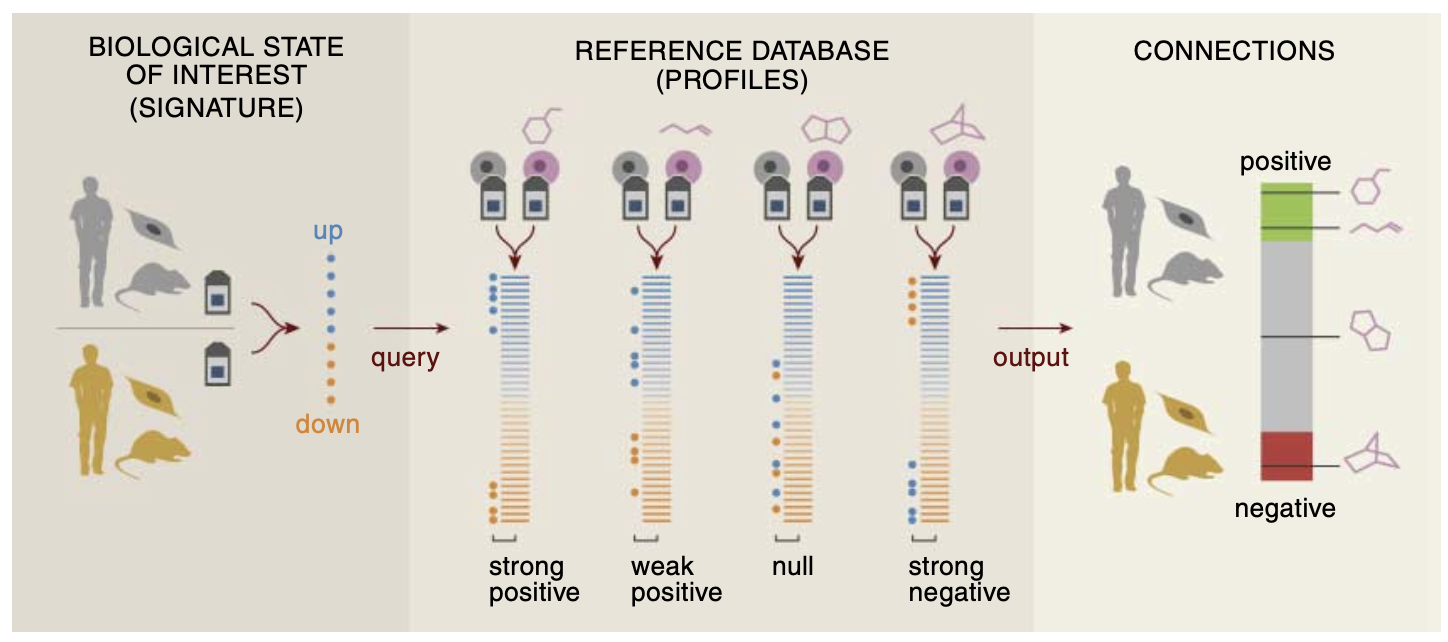
\includegraphics[scale=0.6]{pic_1_sec_3.3.1.png}
    \caption{Принцип метода Connectivity Map}
\end{figure}

На вход данному методу поступает список генов с повышенной экспрессии и список генов с пониженной экспрессией. Списки генов предварительно получают при анализе дифференциальной экспрессии генов между двумя состояниями, например, между здоровой и больной тканью. Далее выполняется запрос в референсную базу данных, где происходит сравнение сигнатуры запроса с известными сигнатурами. Для сигнатур, находящихся в базе данных, известны малые молекулы, способные обратить данную сигнатуру, то есть лекарства, которые могут быть применены для лечения того или иного заболевания, характеризующегося той или иной сигнатурой. После произведенного сравнения метод Connectivity Map выдает ранжированный список молекул с их метриками сходства, на основании которых можно судить о пригодности вещества для обращения сигнатуры.

\par Lamb et. al \cite{lamb2006} описали метод Connectivity Map и провели ряд исследований для валидации предложенного метода. Было показано, что геномные сигнатуры можно использовать для распознавания лекарств с общими механизмами действия. Были найдены известные ингибиторы HDAC и модуляторы рецепторов эстрогена на основе сигнатур. Также было установлено, что метод хорошо работает для обнаружения неизвестных механизмов действия (была предсказана активность гедонина как ингибитора HSP90) и выявления потенциальных новых терапевтических средств (обнаружена способность сиролимуса преодолевать резистентность к дексаметазону при остром лимфобластном лейкозе). Результаты также показывают, что сигнатуры часто сохраняются в различных типах клеток и в различных условиях (сигнатура устойчивости к дексаметазону была определена в образцах костного мозга, но поиск проводился по профилям из линии рака груди MCF7). В то же время результаты демонстрируют ограничения использования только нескольких клеточных линий (сигнатура эстрадиола не была обнаружена в клетках, лишенных рецепторов эстрогена) или только нескольких концентраций (хлорпромазин не распознавался как фенотиазин при 1 мМ).


\subsubsection{Существующий инструмент}
Duan et al. \cite{duan2016} представили инструмент, который называется L1000CDS2, с помощью которого можно произвести Connectivity Map и получить список малых молекул, которые могут обратить вспять или имитировать экспрессионную сигнатуру при болезни и других биологических условиях. Большой набор сигнатур, вычисленных методом CD (Characteristic Direction), предоставляется в виде современного веб-приложения. Помимо определения приоритета малых молекул для того, чтобы обратить или имитировать входную сигнатуру или предварительно вычисленные сигнатуры для 670 заболеваний и набора эндогенных лигандов, веб-инструмент поисковой машины L1000CDS2 также предсказывает попарные комбинации малых молекул, выполняет подструктурный анализ обогащения и вычисляет прогнозируемые цели на основе внешнего набора сигнатур. Так для валидации метода было выполнено предсказание лекарственной молекулы для лечения вируса Эбола на ранних стадиях. Наиболее вероятная молекула, обращающая сигнатуру клеток, инфицированных вирусом Эбола, кенпауллон, как было показано, ослабляет инфекцию дозозависимым образом, не вызывая клеточной токсичности в двух линиях клеток. Были предсказаны задействованные гены-мишени и сигнальные пути клеток, которые указывали на гены иммунного ответа, управляемые ингибированием путей CDK1-2 и GSK3B, и потенциально активирующие передачу STAT сигналов.